\section{Introduction}

\begin{flushright}
We are drowning in information and starving for knowledge.\\
-Rutherford D. Roger
\end{flushright}

Astronomy is entering a Big-Data era \cite{Moravec2019, Siemiginowska2019, Gunn2006a} thanks to advances in computing power, instrumentation, and new telescopes that are paving the way to large astronomical surveys. This explosion in data generation is a trend that is expected to keep growing at an exponential rate in the coming years. For instance, we can mention a couple of the major game-changers in the large survey initiatives: \textbf{The Square Kilometre Array (SKA),} to be built in Australia and South Africa. The SKA is expected to see light by 2027 and it is estimated to generate about an exabyte ($\sim 10^{18}$) of raw data every day \cite{SKAweb, Philip2019}. Another major key player will be \textbf{the Large Synoptic Survey Telescope (LSST)} \cite{Ivezic2019}. Citing from \cite{LSSTweb} web page : 

``The goal of the Large Synoptic Survey Telescope (LSST) project is to conduct a 10-year survey of the sky that will deliver a 500 petabyte set of images and data products that will address some of the most pressing questions about the structure and evolution of the universe and the objects in it." 

A current operating large survey is \textbf{the Sloan Digital Sky Survey (SDSS)} \cite{Gunn2006a, Weijmans2016}. From the \cite{SDSSweb} web site:

``The Sloan Digital Sky Survey has created the most detailed three-dimensional maps of the Universe ever made, with deep multi-color images of one-third of the sky, and spectra for more than three million astronomical objects."

Within all these data, there will lie new scientific truths. With the traditional human-computer paradigm, however, it will be impossible to unveil them. Since the amounts of data to handle will be vast, spotting even a small fraction of them will be unattainable.

%Not to mention how to spot transient phenomena and generate alerts to follow them \cite{Mahabal2019, Patterson2019}.

The new challenges posed by these ``big-data" can be managed using algorithms able to uncover these truths, which are not limited by the aforementioned drawbacks \cite{Baron2017, Reis2019}. Algorithms of these types exist in the realm of Machine Learning (ML) \cite{IvezicBook2014, Aggarwal2017, Geron2017, Patel2019}. ML techniques extract insights and deal with data in a completely different way when compared with traditional approaches.

In the traditional paradigm workflow, the researcher feeds data (\textbf{input}) to a \textbf{program} in order to obtain useful information from it (\textbf{output}) \cite{Sriram}. We can picture this workflow with an illustration \cite{Sriram}:

\begin{figure}[h]
\centering
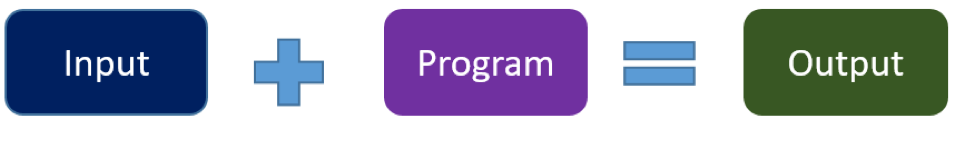
\includegraphics[width=100 mm]{./figures/Traditional-Programming.png}
\caption{\small{Traditional approach}}
\end{figure}

This \textbf{traditional program} is created based on a preconception of the physics behind the phenomena. As a practical example, we can consider the case of fitting the radiated energy by a stellar object as a function of the wavelength. Here the fitting routine will rely on a black-body curve. Several modifications are added to account for additional phenomenologies like the interactions with nearby objects or the material between use and the stellar object. Here we are imposing restriction a priori to our science case. Additionally, there are more drawbacks to using this approach. For instance, it will not scale well for huge amounts of data, and the insights obtained can be misleading because of the complex nature of the data.

Finally, in the ML paradigm, an algorithm is programmed with generic rules, in consequence, it doesn't rely on preconceptions of the phenomenology behind the problem at hand. These rules are so generic, that the same algorithm can be used to study completely different phenomena \cite{Sriram}. The workflow in an ML project can be illustrated as follows:

\begin{figure}[h]
\centering
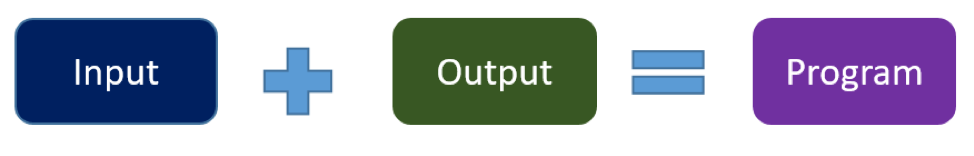
\includegraphics[width=100 mm]{./figures/Machine-Learning.png}
\caption{\small{ML approach}}
\end{figure}

The difference as can be noted from the diagram is that the program is the actual output of the process. In the next section, we'll elaborate more about this process and the reasons why it suits amazingly to deal with the data richness in astronomy. 

As a final remark, we have to be aware that the overall performance of ML techniques improves when data of high quality is feed to the algorithm. The more the data, with better quality, the best the results. The natural conclusion then is that the overall scenario of ML and the data explosion in astronomy makes a perfect target for a highly productive symbiotic relationship between astronomy and Artificial Intelligence (AI).


\subsection{Supervised learning \& Unsupervised learning}

So far we have mentioned the word data quite a lot. Let's make a subtle distinction between data and \textbf{data in the context of training} an ML algorithm: the latter receives the name of the training data-set, aka, \textbf{the training set}. Now, going back to ML, we say that \textbf{Supervised Learning (SL)} happens when the training set is labeled before the training process starts. \textbf{A label} is a fact associated with a data point \textbf{(an instance)}. Therefore in SL, the training set consists of the collection of all instances and their labels. For instance, in \cite{Stensbo-Smidt2017, Delli2019} an SL approach is considered to estimate SFRs using multiband photometry rather than spectroscopic observations from the SDSS DR7. The training set used in both studies is the same. The labels were generated using spectroscopy. As a result, they created programs able to obtain accurate estimates of SFRs using purely multi-band photometric data from the SDSS.

For the case of \textbf{Unsupervised Learning (UL)}, the training set does not contain labels, rather they are added a posteriori once the training has been carried out. In a nutshell, that's the difference between these two approaches. As an example, we have the study case in \cite{Martin2019}, where the authors use a UL approach for morphological ``classification'' of galaxy images. The algorithm in \cite{Martin2019} separates the images in the  HSC-SSP DR1 data-set into 160 clusters of similar morphological types. Afterward, the clusters are labeled by visual inspection \textbf{(labels are assigned a posteriori)}. This intermediate step makes the labor of classification much simpler and possible for huge datasets. Visually classifying every image is an impossible endeavor in these cases. Finally, UL allowed a more refined classification of the galaxies. This fine-tuning will prove to be even harder for the human expert.

One final definition and to add more vocabulary: the collection of all the instances and their associated labels is known as \textbf{the ground true} in the jargon of the ML community. The panorama explained before could lead us to think that we have either SL or UL, but that's only an oversimplification. Far from that, the division is actually blurred since mixed approaches can be considered.
 
\subsection{SL limitations}

After the introduction given above, some red flags must be pointed out inherent to the use of SL techniques. Since the labels are provided in the training set, there is a risk that \textbf{the ground truth might be biased}. If this is the case, once the training is completed, the bias will be propagated in any subsequent use of the program with unseen data. In the case of astronomy, biased trained algorithms will impact the science we do by generating misleading results. The consequences are direr when this scenario comes about in situations involving humans. Since ML is becoming ubiquitous in everyday life, from decision making in human resources departments to decisions in our justice systems, contaminated data will result in unfair treatment and the perpetuation of these unethical behaviors. For instance, we can mention the case of gender and racist biases \cite{Oneil2016}.

Another possible problem to consider when using SL in astronomy is the answer obtained after the algorithm processes data instances that are very dissimilar to the ones used during the training stage. In this case, there is new and valuable information lost \cite{Baron2017, Reis2019}. Finally, another weak point for the case of SL is related to the generation of training sets with updated ground truth to retrain the ML algorithms. This bottle-neck is especially relevant in our times where the pace of data acquisition increases at a staggering rate, and additionally, it is a tendency that will continue in the coming decades.

The weak points stated above can be addressed with UL. The very nature of UL is its key strength. The outcomes from UL programs are less biased if more and more data are used in the training phase because these techniques do not require data labeled a priori. With more data, UL algorithms are able to capture subtle nuances embedded in the training set that enable us to expand the scope of our science, as illustrated in \cite{Martin2019}. 

An obvious advantage of SL over UL is that for SL a performance measure can be established, optimized and used as a guide. That is not the case for UL because there are no labels to compare with. This difference makes the problems to be tackled by each algorithm of a different nature. The case for UL can be framed as: ``There are not either right or wrong answers in UL''. For instance, we could be interested in knowing what novel objects, not present in our lore, are hidden within the data. This kind of science: anomaly detection, is a perfect fit for UL. In anomaly detection, we face the problem of finding rare objects and even objects we don’t know. For rare and unknown objects it is impossible to have representative data containing the corresponding labels of "rare", not to mention the impossibility of the task for "unknown" instances \cite{Norris2017}. Anomaly detection is a very good example of the utility of UL and the fact that it doesn't need labels to proceed. Good examples of this application in astronomy can be found in  \cite{Baron2017, Reis2018a}, where an unsupervised algorithm was used to find some of the most strange objects in SDSS data.

Summarizing, in the supervised case, the labels are known a priori and they drive the learning process. This means that the scope of the knowledge acquired by the algorithm is conditioned to the relations encoded in the ground truth already known. In the case of unsupervised learning, the algorithm finds itself the underlying relations, and the labels are added a posteriori to obtain the ground truth. In the end, and despite the differences between the two approaches, one key factor and one of great importance, is the quality of the data. All the knowledge we want to extract will come from the data, therefore it is compelling for the data to be of high quality.

\subsection{Knowledge Discovery}

The end goal of these tools is knowledge discovery from the data, a term that is used in the fields of data mining and ML \cite{IvezicBook2014}. To accomplish this, we need to make a working model for the data that allow us to make predictions and also to better understand the physics behind the data: either quantitatively or qualitatively. These techniques are highly promising but it is important to remember that a model is only a representation of reality and that reality is more complex. Therefore, we need to be careful about the scope and limitations of the models we use. As an example, we can consider two very different approaches when modeling some data:

\begin{enumerate}
    \item A linear model: one-parameters model
    \item A polynomial model: n-parameter model,
\end{enumerate}

The case for a linear behavior is a very strong assumption about the phenomenology that could lead to a poor interpretation of the problem if it has a higher degree of complexity. On the other hand, an n-degree polynomial could overfit the data, leading to a poor predictive power, in consequence, the model doesn't generalize well for points outside the training data. There is always a trade-off between the variance and the bias inherent to the complexity of the model \cite{Hastie2009}, these, therefore, constitute the scope and limitations of a model when dealing with knowledge discovery from data.
